\mbox{$\displaystyle -\,\frac{1}{2}$\,
\begin{tikzpicture}[x=0.340cm, y=0.340cm, line width=0.420pt, baseline={([yshift=-0.6ex]0,0)}]
  \draw (-0.500,0.000) arc[start angle=186.026, end angle=353.974, radius=0.503];
  \fill (0.378,-0.300) -- (0.122,-0.347) -- (0.243,-0.389) -- (0.235,-0.517) -- cycle;
  \fill (-0.378,-0.300) -- (-0.235,-0.517) -- (-0.243,-0.389) -- (-0.122,-0.347) -- cycle;
  \draw plot[smooth, tension=0.7] coordinates {(-0.500,0.000) (-0.450,0.076) (-0.400,0.108) (-0.350,0.076) (-0.300,0.000) (-0.250,-0.076) (-0.200,-0.108) (-0.150,-0.076) (-0.100,0.000) (-0.050,0.076) (0.000,0.108) (0.050,0.076) (0.100,0.000) (0.150,-0.076) (0.200,-0.108) (0.250,-0.076) (0.300,0.000) (0.350,0.076) (0.400,0.108) (0.450,0.076) (0.500,0.000)};
  \draw (-0.500,0.000) arc[start angle=173.974, end angle=6.026, radius=0.503];
  \fill (-0.248,0.401) -- (-0.493,0.317) -- (-0.367,0.293) -- (-0.357,0.165) -- cycle;
  \fill (0.248,0.401) -- (0.357,0.165) -- (0.367,0.293) -- (0.493,0.317) -- cycle;
  \fill (-0.500,0.000) circle (0.064);
  \fill (0.500,0.000) circle (0.064);
\end{tikzpicture}}
\diagramgap
\mbox{$\displaystyle +\,\frac{1}{2}$\,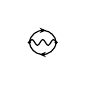
\begin{tikzpicture}[x=0.340cm, y=0.340cm, line width=0.420pt, baseline={([yshift=-0.6ex]0,0)}]
  \draw (0.500,0.000) arc[start angle=353.974, end angle=186.026, radius=0.503];
  \fill (-0.119,-0.450) -- (0.119,-0.552) -- (0.042,-0.450) -- (0.119,-0.348) -- cycle;
  \draw plot[smooth, tension=0.7] coordinates {(-0.500,0.000) (-0.450,0.076) (-0.400,0.108) (-0.350,0.076) (-0.300,0.000) (-0.250,-0.076) (-0.200,-0.108) (-0.150,-0.076) (-0.100,0.000) (-0.050,0.076) (0.000,0.108) (0.050,0.076) (0.100,0.000) (0.150,-0.076) (0.200,-0.108) (0.250,-0.076) (0.300,0.000) (0.350,0.076) (0.400,0.108) (0.450,0.076) (0.500,0.000)};
  \draw (-0.500,0.000) arc[start angle=173.974, end angle=6.026, radius=0.503];
  \fill (0.119,0.450) -- (-0.119,0.552) -- (-0.042,0.450) -- (-0.119,0.348) -- cycle;
  \fill (-0.500,0.000) circle (0.064);
  \fill (0.500,0.000) circle (0.064);
\end{tikzpicture}}
\diagramgap
\mbox{$\displaystyle -\,\frac{1}{2}$\,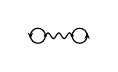
\begin{tikzpicture}[x=0.340cm, y=0.340cm, line width=0.420pt, baseline={([yshift=-0.6ex]0,0)}]
  \draw plot[smooth, tension=0.7] coordinates {(-0.500,0.000) (-0.450,0.076) (-0.400,0.108) (-0.350,0.076) (-0.300,0.000) (-0.250,-0.076) (-0.200,-0.108) (-0.150,-0.076) (-0.100,0.000) (-0.050,0.076) (0.000,0.108) (0.050,0.076) (0.100,0.000) (0.150,-0.076) (0.200,-0.108) (0.250,-0.076) (0.300,0.000) (0.350,0.076) (0.400,0.108) (0.450,0.076) (0.500,0.000)};
  \draw (-0.500,0.000) arc[start angle=0.000, end angle=360.000, radius=0.280];
  \fill (-1.060,-0.119) -- (-0.958,0.119) -- (-1.060,0.042) -- (-1.162,0.119) -- cycle;
  \draw (0.500,0.000) arc[start angle=180.000, end angle=540.000, radius=0.280];
  \fill (1.060,0.119) -- (0.958,-0.119) -- (1.060,-0.042) -- (1.162,-0.119) -- cycle;
  \fill (-0.500,0.000) circle (0.064);
  \fill (0.500,0.000) circle (0.064);
\end{tikzpicture}}
